\chapter{Evaluation}
\label{chap:Evaluation}

\section{Section1}
\paragraph{paragraph1}
\subsection{Features}
Dans une tâche d'object detection, nous utilisons le score IoU qui signifie Intersection over Union.
C'est un score qui compare les bounding boxes prédites par le modèle avec les bounding boxes réels (ground-truth).
\begin{figure}[tbh!]
    \centering
    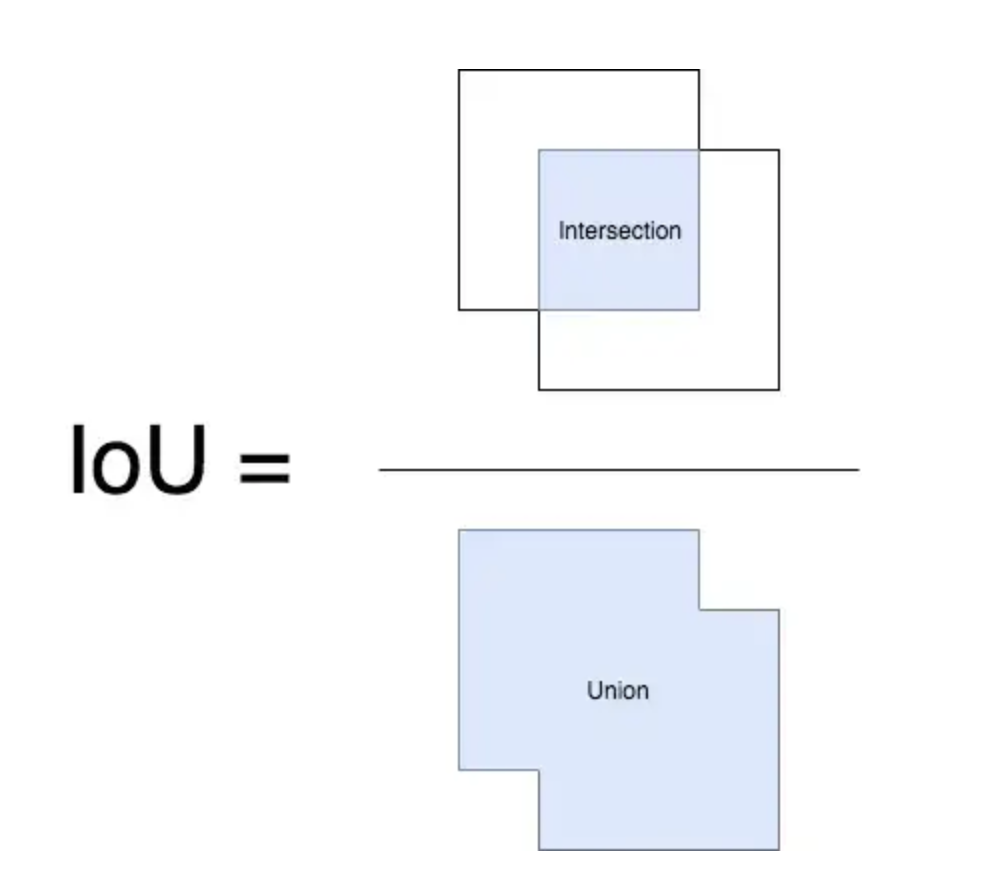
\includegraphics[width=\textwidth]{images/iou.png}
    \caption{Intersection over Union}
    \label{fig:iou}
\end{figure}
Une tâche d'object detection comprend deux sous-problèmes: la classification et la localisation.
Ainsi nous avons plusieurs métriques pour analyser la performance d'un modèle. IoU se concentre sur l
a localisation des bounding box prédites tandis que la métrique mAP (mean Average Precision) 
se concentre sur la classification.

% -- Vic : 

\section{Évaluations des deux modèles sélectionnés}

Après avoir testé plusieurs approches comme mentionnées dans le chapitre \autoref{chap:Modeles}, nous avons retenu - comme mentionné également au chapitre 6 - deux modèles dont nous allons ici comparer les scores d'évaluation :

\begin{itemize}
    \item[-] Faster R-CNN avec Detectron2 et
    \item[-] Retinanet avec Detectron2.
\end{itemize}

Voici donc un tableau résumant les average precision (AP) scores de chaque catégorie suivant le treshold, ainsi 

Scores par classe : 

\begin{center}
   \begin{tabular}{ | l | l || c |}
     \hline
     modèle & catégorie & AP score \\ \hline
     \multirow Faster R-CNN & crapaud-grenouille & 42.03 \\ 
     & triton & 42.58   \\ \hline
     \multirow Retinanet & crapaud-grenouille & 49.40 \\
     & triton & 0.00 \\
     \hline
   \end{tabular}
 \end{center}

 Bien que le score pour la classe crapaud-grenouille soit plus élevé à l'aide du modèle Retinanet, le score pour la classe triton est de zéro. Rappelons que la tâche initiale de ce projet est de compter le nombre de triton/crapaud-grenouille qui utilisent les crapauduc ; ainsi, nous avons choisi l'algorithme Faster R-CNN comme modèle final pour cette tâche de classification.

\subsection{Modèle final choisi}

\paragraph{Entraînement}

Voici donc comment nous avons premièrement entraîné notre modèle Faster R-CNN, avec Detectron 2 : 

\lstset{language=Python}
\begin{lstlisting}
cfg = get_cfg()
cfg.merge_from_file(model_zoo.get_config_file("COCO-Detection/
faster_rcnn_X_101_32x8d_FPN_3x.yaml"))
cfg.DATASETS.TRAIN = ("triton_train",)
cfg.DATASETS.TEST = ()
cfg.DATALOADER.NUM_WORKERS = 2
cfg.MODEL.WEIGHTS = model_zoo.get_checkpoint_url("COCO-Detection/
faster_rcnn_X_101_32x8d_FPN_3x.yaml")  
cfg.SOLVER.IMS_PER_BATCH = 2 
cfg.SOLVER.BASE_LR = 0.00020 
cfg.SOLVER.MAX_ITER = 500 
cfg.SOLVER.STEPS = []   
cfg.MODEL.ROI_HEADS.BATCH_SIZE_PER_IMAGE = 128  
cfg.MODEL.ROI_HEADS.NUM_CLASSES = 4 
\end{lstlisting}


\paragraph{Test}

Et voici donc le modèle construit pour tester nos données d'évaluation : 

\lstset{language=Python}
\begin{lstlisting}
# on recuperation des poids du modele qu'on vient d'entrainer
cfg.MODEL.WEIGHTS = os.path.join(cfg.OUTPUT_DIR, "model_final.pth")  
# determination d'un treshold pour le test
cfg.MODEL.ROI_HEADS.SCORE_THRESH_TEST = 0.7  
# construction du predicteur
predictor = DefaultPredictor(cfg)
\end{lstlisting}\newline\newline

Le treshold choisi pour le test ci-dessus indique donc qu'on considérera une image comme étant prédite d'une certaine classe si le modèle est sûr à au moins 70\% de sa classification.\newline

Voici deux exemples de résultats de classification par notre modèle ainsi créé :

\begin{figure}[H]
    \centering
    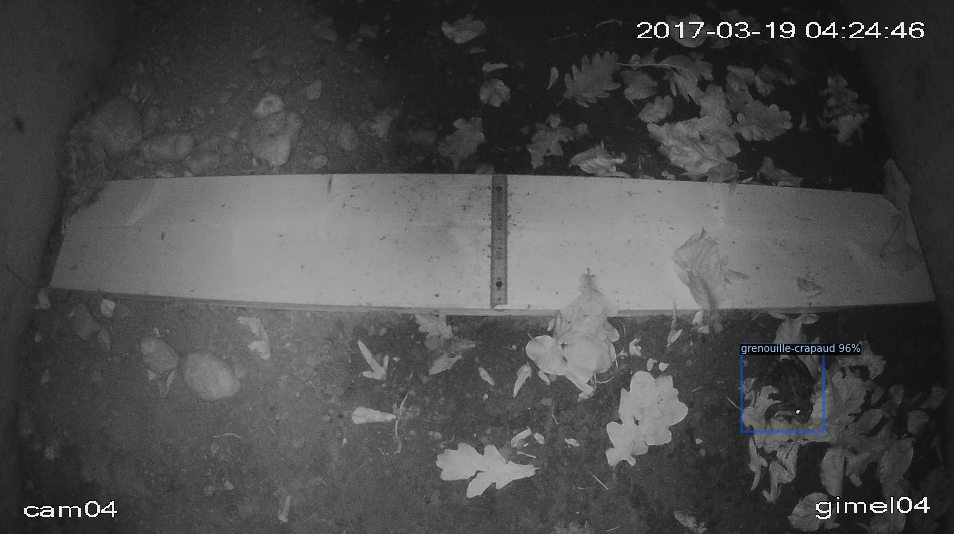
\includegraphics[width=300px]{images/Eval_FasterRCNN_crapGren.png}
    \caption{Prédiction de Faster R-CNN - crapaud-grenouille}
    \label{fig:fasterRcnn_crapGren}
\end{figure}

\begin{figure}[H]
    \centering
    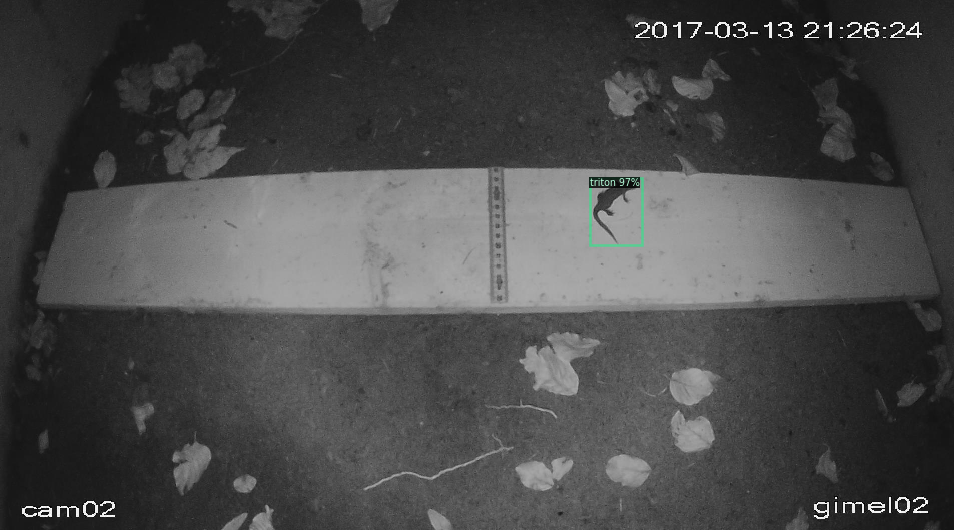
\includegraphics[width=300px]{images/Eval_FasterRCNN_triton.png}
    \caption{Prédiction de Faster R-CNN - triton}
    \label{fig:fasterRcnn_triton}
\end{figure}

Validation (résultats) important de dire que images sont similaires à celles deja vues blabla --> Joris (précision sur ce qui est dit..)

